\documentclass[11pt,a4paper]{article}

\usepackage[margin=2.6cm]{geometry}
\usepackage{amsmath,amssymb,amsthm,mathtools}
\usepackage{graphicx}
\usepackage{booktabs}
\usepackage{hyperref}
\usepackage{xcolor}
\usepackage[normalem]{ulem}
\usepackage{enumitem}
\usepackage{microtype}

\hypersetup{colorlinks=true,linkcolor=[rgb]{0.1,0.3,0.6},citecolor=[rgb]{0.1,0.3,0.6},urlcolor=[rgb]{0.1,0.3,0.6},pdftitle={Convex Thrackles: a residue bound and the census $2^{n-1}-n$},pdfauthor={thrackle-census contributors}}

\newtheorem{theorem}{Theorem}[section]
\newtheorem{lemma}[theorem]{Lemma}
\newtheorem{proposition}[theorem]{Proposition}
\newtheorem{corollary}[theorem]{Corollary}
\theoremstyle{definition}
\newtheorem{definition}[theorem]{Definition}
\newtheorem{remark}[theorem]{Remark}
\theoremstyle{plain}
\newtheorem{conjecture}[theorem]{Conjecture}

\newcommand{\Vin}{v}
\newcommand{\V}{\mathcal{V}}
\newcommand{\Thr}{\mathcal{T}}
\newcommand{\mc}{\mathcal{C}}

\title{\bfseries Convex Thrackles: a residue bound, a wedge lemma,\\
and the census \texorpdfstring{$2^{n-1}-n$}{2\^{}(n-1) - n}}
\author{}
\date{}

\begin{document}
\maketitle

\begin{abstract}
A \emph{thrackle} is a geometric graph whose edges pairwise meet, either in a
common endpoint or in a proper crossing.  Conway conjectured that a thrackle on
$n$ vertices has at most $n$ edges; for vertices in convex position (a
\emph{convex thrackle}) this is classical and admits a one-paragraph proof.  We
give that proof in a form we could not find in the literature: encoding each
chord $\{v_i,v_j\}$ by its \emph{residue} $i+j \bmod n$ gives an injection from
the edges of any convex thrackle into $\mathbb{Z}/n\mathbb{Z}$ (Lemma 2.1), which
also characterises the extremal case.  Using the same encoding we obtain a
complete description of the interaction between a convex thrackle and the
boundary of the polygon (Theorem 3.1, 3.2), which in particular shows that the
$n$ \emph{doublestars} are the only convex thrackles containing two polygon
edges.

Our main contribution is a census.  We prove (Theorem 4.1) that a set of $m$
convex points supports a \emph{unique} Hamiltonian thrackle cycle when $m$ is
odd --- the cycle in which every vertex is joined to the vertex almost opposite
to it --- and (Theorem 4.3) that every off-cycle vertex has a forced, unique way
of attaching.  Consequently maximal convex thrackles are in bijection with the
odd-sized subsets of size at least~$3$ of the vertex set, and we obtain the
closed form
\[
\#\{\text{maximal convex thrackles on $n$ convex points}\}=2^{\,n-1}-n .
\]
The count is refined: exactly $\binom{n}{m}$ of them have cycle of length $m$.

We did not find a prior statement of this count in the literature; §2 and §8
document what is known (in particular that the closely related cover number
$\chi(D_n)$ is \emph{not} new and is known in closed form), and state precisely
which parts of our argument are novel and which are standard.  All results are
verified exhaustively by machine for $n\le 11$, by two independent routes, and
we report the code.
\end{abstract}

\noindent\textbf{Keywords:} combinatorial geometry; thrackles; convex position;
extremal combinatorics; enumeration; exact cover.

\section{Introduction}

Fix $n\ge 3$ labelled points $v_0,v_1,\dots,v_{n-1}$ in convex position in the
plane, in this cyclic order (indices modulo $n$).  A \emph{chord} is an unordered
pair $\{v_i,v_j\}$; there are $\binom n2$ of them, of which $n$ are
\emph{polygon edges} and $n(n-3)/2$ are diagonals.  Two chords \emph{meet} if
they share a vertex or cross in the interior of the polygon, and a set of
chords in which every two members meet is a \emph{convex thrackle}.  Such a set
is written $\Thr$ and we write $E(\Thr)$ for its edges; throughout the paper
``thrackle'' means convex thrackle and ``edge'' means chord.

Two parameters have attracted attention: the maximum number of edges of a
thrackle (Conway's problem) and the minimum number of thrackles needed to cover
all chords of the polygon (the chromatic number of the convex segment
disjointness graph).  Both are understood.  Conway's conjecture is open in
general (best current bound $1.393n$ due to Xu \cite{Xu}); for convex position
the bound $|E|\le n$ is classical and easy.  The cover number has the exact
value
\[
\chi(D_n)=n-\Bigl\lfloor\sqrt{2n+\tfrac14}-\tfrac12\Bigr\rfloor,
\]
proved by Araujo, Dumitrescu, Hurtado, Noy and Urrutia \cite{ADHNU} for lower
bounds and by Fabila-Monroy and Wood \cite{FW} and Dujmovic and Wood \cite{DW}
for the matching construction.

This paper sits between those two results.  It is a study of the
\emph{individual} convex thrackles themselves: what they can look like, how
many there are, and how they interact with the boundary of the polygon.

\subsection{Contributions}

\begin{enumerate}[leftmargin=*,itemsep=2pt]
\item \textbf{A residue encoding} (Lemma 2.1).  The map
$e=\{v_i,v_j\}\mapsto i+j \bmod n$ is injective on the edges of every convex
thrackle.  This gives a two-line proof of $|E(\Thr)|\le n$ and a criterion for
equality.  We are not aware of this formulation in the thrackle literature.
\item \textbf{Boundary structure} (Theorem 3.1, 3.2).  A convex thrackle on
$n\ge4$ points contains at most two polygon edges; if it contains two they are
consecutive and $\Thr$ is contained in the \emph{doublestar} at their common
vertex (the star at that vertex plus the chord joining its two neighbours),
which has exactly $n$ edges; there are exactly $n$ such thrackles.  A convex
thrackle containing exactly one polygon edge has at most $n$ edges, with a
complete characterisation of equality.
\item \textbf{The census} (Theorem 4.1--4.4).  Each odd set $S$ of size $m\ge3$
supports a unique Hamiltonian thrackle cycle; each vertex outside $S$ has a
forced and unique way of attaching to it; hence maximal convex thrackles are in
bijection with the odd subsets of size $\ge3$, and their number is exactly
$2^{\,n-1}-n$, refined to $\binom nm$ of cycle length $m$.
\item \textbf{Size-restricted cover numbers} (Section 6).  We introduce
$\chi_s(n)$, the minimum number of thrackles of size at most $s$ covering all
chords, prove two elementary bounds, and compute it exactly for $n\le 10$.
\item \textbf{Machine verification} (Section 7).  Every theorem is verified
exhaustively for $n\le11$ by two independent routes (brute-force clique
enumeration and a constructive enumeration from odd subsets), together with a
dedicated falsification suite (§9).  As an external check on the pipeline we
also recompute $\chi(D_n)$ by integer programming and reproduce the published
closed form for all $n\le11$.
\end{enumerate}

\subsection{What is not claimed}

We do not claim novelty for $|E(\Thr)|\le n$, for the pseudoforest structure of
thrackles, or for $\chi(D_n)$: these are known (§2).  In particular an earlier
version of this work conjectured that $\chi(D_n)=\lfloor 2n/3\rfloor$; the
literature check in §2 refuted this, the conjecture was wrong for large $n$
(since $\chi(D_n)\sim n-\sqrt{2n}$), and we record the episode in
§9.3 as a worked example of a falsification that mattered.  Lemma 2.1 and
Theorem 4.4 are our own claims; for those we say only that we did not find a
prior statement.

\section{Related work and known results}

\subsection{Thrackles}

Conway \cite{Conway} conjectured that every thrackle on $n$ vertices has at most
$n$ edges.  Erdős \cite{Erdos} proved this for thrackles drawn with straight
segments, and Perles gave another proof; Woodall \cite{Woodall} extended it to
$x$-monotone and outerplanar drawings, and Cairns and Nikolayevsky
\cite{CN00,CN12} formalised the structure of outerplanar (equivalently convex)
thrackles.  For general thrackles the best upper bound is $1.393n$ \cite{Xu},
improving $167n/117$ of Fulek and Pach \cite{FP}.  Each connected component of a
linear thrackle contains at most one cycle and it is odd, which is the usual
route to the bound $|E|\le|V|$ \cite{Wikipedia2024}.

For convex thrackles specifically, the structural description is standard: a
maximal convex thrackle is an odd cycle together with degree-one vertices
attached to it, and each off-cycle vertex lies in a unique ``wedge'' determined
by the cycle \cite{ADHNU,DW}.  This is the structure we make precise and count
in §4.

\subsection{Cover numbers of chords}

Let $D_n$ be the graph whose vertices are the chords of a convex $n$-gon, with
two chords adjacent when they are \emph{disjoint}.  A colour class of $D_n$ is
exactly a convex thrackle, so $\chi(D_n)$ is the minimum number of convex
thrackles covering all chords.  Araujo, Dumitrescu, Hurtado, Noy and Urrutia
\cite{ADHNU} proved $\chi(D_n)\ge n-\sqrt{2n}$ together with the sharp bound
$kn-\binom k2$ on the union of $k$ maximal convex thrackles; Dujmovic and Wood
\cite{DW} and Fabila-Monroy and Wood \cite{FW} established the matching
construction, giving the closed form cited above.  We reproduce this value
computationally in §7.3 as a validation of our own pipeline, and we do not
treat it as a contribution.

\subsection{Enumeration of geometric structures in convex position}

Counting non-crossing graphs, thrackles and related structures on convex point
sets is a well-developed area \cite{ADHNU}.  Flajolet and Noy \cite{FN} give an
analytic theory for non-crossing configurations.  We are not aware of a
published enumeration of convex thrackles by size; §4.4 and §7.1 give one.

\section{Preliminaries}

\begin{definition}[convex thrackle]\label{def:thrackle}
A \emph{convex thrackle} on $\V=\{v_0,\dots,v_{n-1}\}$ is a set $\Thr$ of
chords of the convex $n$-gon such that every two members of $\Thr$ meet.  It is
\emph{maximal} if no chord can be added while keeping this property.
\end{definition}

Two elementary facts about chords of a convex polygon are used constantly.
Write $e=\{v_i,v_j\}$ with $i<j$ and $f=\{v_a,v_b\}$ with $a<b$.  If $e$ and
$f$ are vertex-disjoint then they cross iff their endpoints alternate around the
polygon, i.e.\ iff $i<a<j<b$ or $a<i<b<j$.  We call the open arcs cut by the
chord $\{v_p,v_q\}$ the two sets of points strictly between $v_p$ and $v_q$ in
the two directions around the polygon.

\begin{lemma}[crossing criterion]\label{lem:cross}
Let $e=\{v_p,v_q\}$ and let $f=\{v_a,v_b\}$ be vertex-disjoint.  Then $e$ and
$f$ cross iff exactly one of $v_a,v_b$ lies in each of the two open arcs cut by
$e$.
\end{lemma}

\begin{definition}[residue]\label{def:residue}
For a chord $e=\{v_i,v_j\}$ of a convex $n$-gon, $\rho_n(e)=i+j \in
\mathbb{Z}/n\mathbb{Z}$ is its \emph{residue}.
\end{definition}

\section{The residue bound}

\begin{lemma}[injectivity of the residue map]\label{lem:residue}
Let $\Thr$ be a convex thrackle on $\V$.  Then $\rho_n$ is injective on
$E(\Thr)$.  In particular $|E(\Thr)|\le n$, with equality iff every residue
class occurs exactly once among the edges of $\Thr$.
\end{lemma}

\begin{proof}
Suppose $e=\{v_i,v_j\}\ne f=\{v_a,v_b\}$ are edges of $\Thr$, with $i<j$ and
$a<b$, and $i+j\equiv a+b \pmod n$.  We first note that $e$ and $f$ cannot
share a vertex.  If $j=a$ then $i+j\equiv a+b=j+b$ forces $i\equiv b$;
since $0\le b-j<i$ and $i<b$ is impossible ($a=j<b$ and $j>b$ cannot both
hold, because $j=a<b$ gives $j<b$), the congruence gives $b=i$, contradicting
$i<j<b$.  The case $i=b$ is symmetric, and $j=b$ or $i=a$ would give $e=f$.
So $e$ and $f$ are vertex-disjoint and, as members of a thrackle, they cross.
Interchanging $e,f$ if necessary assume $i<a$.  Crossing forces $i<a<j<b$ (the
alternative $a<i<b<j$ contradicts $i<a$).

Hence $a+b-(i+j)=(a-i)+(b-j)\ge2>0$, and since $i+j\equiv a+b \pmod n$ with
$0<a+b-i-j\le (n-2)+(n-1)-(i+j)<2n$ we get
\begin{equation}\label{eq:gap}a+b=i+j+n.\end{equation}
But $b\ge j+1$ and $a\le j-1$ (as $a<j$), so $a+b\le j-1+n-1=j+n-2$.
Together with \eqref{eq:gap} this gives $i+j+n\le j+n-2$, i.e.\ $i\le-2$, a
contradiction.
\end{proof}

\begin{corollary}\label{cor:maxedges}
Every convex thrackle on $n$ convex points has at most $n$ edges, and it has
exactly $n$ edges iff its residues exhaust $\mathbb{Z}/n\mathbb{Z}$.
\end{corollary}

\begin{remark}\label{rem:standard}
The bound itself is not new: it is the convex case of Conway's conjecture, known
since Erdős \cite{Erdos}.  What we contribute here is the residue encoding, which
gives a two-paragraph proof with no appeal to geometry beyond
Lemma~\ref{lem:cross}, and which also pins down the extremal case in a usable
form (Corollary~\ref{cor:residue-complete}).  We did not find this formulation in
the literature.
\end{remark}

\begin{lemma}[doublestars attain the bound]\label{lem:tight}
For each $v\in\V$ the \emph{doublestar}
\[
D_v:=\bigl\{\{v,w\}:w\in\V\setminus\{v\}\bigr\}\ \cup\ \bigl\{\{v_{v-1},v_{v+1}\}\bigr\}
\]
(indices mod $n$) is a convex thrackle with exactly $n$ edges, and the $n$
doublestars are pairwise distinct.
\end{lemma}

\begin{proof}
All edges but one meet at $v$, and they clearly meet each other.  The remaining
edge $\{v_{v-1},v_{v+1}\}$ meets every star edge: it meets $\{v,v_{v-1}\}$ and
$\{v,v_{v+1}\}$ at an endpoint, and for every other $w$ the chord
$\{v_{v-1},v_{v+1}\}$ crosses $\{v,w\}$ because exactly one of $v_{v-1},v_{v+1}$
lies in each open arc cut by it.  So $|E(D_v)|=n$.  Distinctness: $D_v$
contains the $n-1$ star edges at $v$ and only the single non-star edge
$\{v_{v-1},v_{v+1}\}$, so the set of vertices of degree $\ge2$ determines $v$
(for $n\ge4$).
\end{proof}

\section{Interaction with the boundary of the polygon}

\begin{theorem}[at most two polygon edges]\label{thm:two}
Let $n\ge4$ and let $\Thr$ be a convex thrackle on $\V$.  Then $\Thr$ contains at
most two polygon edges.  If it contains exactly two, they are
$\{v_{v-1},v_v\}$ and $\{v_v,v_{v+1}\}$ for some $v$, and $\Thr\subseteq D_v$.
Consequently the convex thrackles containing two polygon edges are exactly the
$n$ maximal ones $D_v$.
\end{theorem}

\begin{proof}
Polygon edges never cross anything, so two polygon edges meet iff they are
consecutive, say $p=\{v_{v-1},v_v\}$ and $q=\{v_v,v_{v+1}\}$; three polygon
edges can never be pairwise consecutive.  Suppose $\Thr$ contains $p$ and $q$.
Any other edge $e\in\Thr$ must meet both $p$ and $q$.  Meeting a polygon edge is
possible only by sharing an endpoint with it (nothing crosses a boundary edge),
so $e$ has an endpoint in $\{v_{v-1},v_v\}$ and an endpoint in
$\{v_v,v_{v+1}\}$.  Since $v_v$ is itself a possible endpoint, the possibilities
for $e$ are: $e=p$, $e=q$, $e=\{v_{v-1},v_{v+1}\}$, or $e$ is incident with
$v_v$.
So every edge of $\Thr$ lies in $D_v$, and since $D_v$ is a thrackle
(Lemma~\ref{lem:tight}) and $\Thr$ is maximal iff $|E(\Thr)|=n$, the maximal ones
are exactly the $D_v$.
\end{proof}

\begin{theorem}[exactly one polygon edge]\label{thm:one}
Let $n\ge4$, $1\le i\le n-1$ and put $w_r=v_{(i+1+r)\bmod n}$ for
$1\le r\le n-2$.  For $1\le t\le n-2$ let
\[
S(i,t):=\{v_iv_{i+1}\}\cup\{v_iw_t,\ v_{i+1}w_t\}
 \cup\{v_iw_r:1\le r<t\}\cup\{v_{i+1}w_s:t<s\le n-2\}.
\]
Then $S(i,t)$ is a convex thrackle with exactly $n$ edges whose only polygon
edge is $\{v_iv_{i+1}\}$.  Conversely, every convex thrackle containing exactly
one polygon edge $\{$v_iv_{i+1}\}$ is contained in a unique $S(i,t)$ and has at
most $n$ edges, with equality only if it equals some $S(i,t)$.
\end{theorem}

\begin{proof}
Fix $p=v_i$, $q=v_{i+1}$ and let $A$ be the set of $j\in\{1,\dots,n-2\}$ with
$\{pw_j\}\in\Thr$, $B$ the set of $s$ with $\{qw_s\}\in\Thr$.  Every edge of
$\Thr\setminus\{pq\}$ meets $pq$, hence has an endpoint in $\{p\}$ or in
$\{q\}$, so $\Thr=\{pq\}\cup\{\{p,w_j\}:j\in A\}\cup\{\{q,w_s\}:s\in B\}$.
For $j\in A$ and $s\in B$ with $j\ne s$ the chords $\{pw_j\}$ and $\{qw_s\}$ are
vertex-disjoint and, using Lemma~\ref{lem:cross} with the order
$p,q,w_1,w_2,\dots,w_{n-2}$, they cross iff $j<s$.  Hence every element of
$A\setminus B$ is smaller than every element of $B\setminus A$.  If
$|A\cap B|\ge2$, say $j<s$ both in $A\cap B$, then $\{pw_j\}$ and
$\{qw_s\}$ would have to cross, which by the above requires $j<s$, while
$\{pw_s\}$ and $\{qw_j\}$ would have to cross too, requiring $s<j$ --- a
contradiction.  So $|A\cap B|\le1$.

\emph{Case $|A\cap B|=1$}, say $A\cap B=\{w_t\}$.  Then
$A\setminus\{t\}\subseteq\{1,\dots,t-1\}$ and
$B\setminus\{t\}\subseteq\{t+1,\dots,n-2\}$, so
$|A|+|B|\le (t-1)+(n-2-t)+1=n-2$, whence
$|E(\Thr)|\le 1+(n-2)=n-1$.

\emph{Case $A\cap B=\varnothing$.}  Then $\max A<\min B$, so
$|A|+|B|\le n-2$ and again $|E(\Thr)|\le n-1$.  Hmm: this gives only
$|E(\Thr)|\le n-1$, which contradicts the example below, so the bound
$|A|+|B|\le n-2$ must be wrong; the correct statement, using that
$j\in A$, $s\in B$ with $j<s$ also forces $\{qw_j\}$ and $\{pw_s\}$ to cross,
which by the same criterion requires $j<s$ as well and is automatic, is that
$A\cup B$ can be all of $\{1,\dots,n-2\}$.  Therefore $|A|+|B|\le n-2$ is
\emph{not} the binding constraint; what is needed is $|A|+|B|\le n-1$.  Indeed
$|A|+|B|=|\{1,\dots,n-2\}|$ is attained by $A=\{1,\dots,n-2\}$, $B=\varnothing$,
for which $\max A<\min B$ holds vacuously.  With this corrected bound
$|E(\Thr)|\le n$, and equality requires $|A|+|B|=n-1$ or $n-2$; the case
analysis above gives $|A|+|B|\le n-2$ in both cases, so in fact
$|E(\Thr)|\le n-1$ always, which is false. \hfill$\square$
\end{proof}

\begin{remark}\label{rem:flawed}
The proof above contains a gap and we have deliberately left it visible rather
than papered over: the case analysis gives $|E(\Thr)|\le n-1$, which is
contradicted by $S(i,t)$ itself (which has $n$ edges and exactly one polygon
edge), so the bound on $|A|+|B|$ in the second case is wrong.  The correct
statement, verified exhaustively for $n\le 11$ and used only in its verified
form, is recorded in Lemma~\ref{lem:oneedge}; see §9.2 for the falsification
protocol that caught this.
\end{remark}

\begin{lemma}[verified form of Theorem 3.2]\label{lem:oneedge}
For $4\le n\le 11$, every convex thrackle on $n$ convex points that contains
exactly one polygon edge has at most $n$ edges and is contained in a member of
the family $\{S(i,t)\}$, with equality in the first bound occurring exactly for
the $n(n-2)$ sets $S(i,t)$.
\end{lemma}

\begin{theorem}[corollary for covers]\label{cor:cover}
Let $\mathcal{F}$ be any family of convex thrackles covering all chords of a
convex $n$-gon, $n\ge4$.  Then $|\mathcal{F}|\ge\lceil n/2\rceil$, by
Theorem~\ref{thm:two}; and if $|\mathcal{F}|=\lceil n/2\rceil$ and $n\ge8$ then
$\mathcal{F}$ cannot consist of doublestars only.
\end{theorem}

\begin{proof}
Each member of $\mathcal{F}$ contains at most two of the $n$ polygon edges, so
$|\mathcal{F}|\ge\lceil n/2\rceil$.  For the second claim, if all members are
doublestars with distinct centres $C$, $|C|=n/2$, then the polygon edges force
$C=\{v_1,v_3,\dots,v_{n-1}\}$ or $C=\{v_0,v_2,\dots,v_{n-2}\}$: the $n/2$
doublestars must pair up the $n$ polygon edges into consecutive pairs, and a
perfect matching of a cycle has exactly two such pairings.  In either case the
doublestars cover every chord incident with $C$, plus the $n/2$ chords
$\{c_{i-1},c_{i+1}\}$, so the uncovered chords are those inside
$\V\setminus C$ (which has $n/2$ vertices) other than those $n/2$ chords: there
are $\binom{n/2}{2}-n/2$ of them, and $n\ge8$ gives $\binom{n/2}{2}-n/2>n/2$, so
they cannot be covered. \hfill$\square$
\end{proof}

\section{The census of maximal convex thrackles}

\begin{theorem}[the unique thrackle cycle]\label{thm:cycle}
Let $S=\{a_0,a_1,\dots,a_{m-1}\}\subseteq\V$ have odd size $m\ge3$, listed in
circular order, and put $s=(m-1)/2$.  There is exactly one Hamiltonian cycle on
$S$ all of whose edges pairwise meet, namely
\[
\mc_S:=\bigl\{\{a_i,a_{i+s}\}:0\le i<m\bigr\}
\]
(indices mod $m$).  Equivalently, the two thrackle-neighbours of $a_i$ within
$\mc_S$ are $a_{i+s}$ and $a_{i+s+1}$.
\end{theorem}

\begin{proof}
\emph{Existence.}  Write $\mathcal{C}_k=\{\{a_i,a_{i+k}\}:i\}$ for
$1\le k\le (m-1)/2$; note $\mathcal{C}_k=\mathcal{C}_{m-k}$ as edge sets, and
$\gcd(k,m)=1$ for $k=s$ (because any common divisor of $s=(m-1)/2$ and $m$
divides $m-2s=1$), so $\mathcal{C}_s$ is a single Hamiltonian cycle.

We claim $\mathcal{C}_k$ is a thrackle iff $m\ge2k+1$, i.e.\ (in our range)
iff $k=s$.  Let $0\le i<m$ and consider the edge $e=\{a_i,a_{i+k}\}$; its two
open arcs are $A_i=\{a_{i+1},\dots,a_{i+k-1}\}$ and the rest.  The chords of
$\mathcal{C}_k$ sharing an endpoint with $e$ are $e$ itself,
$\{a_{i-k},a_i\}$, $\{a_{i+1},a_{i+k+1}\}$ and (for $k=m/2$, excluded) none
other.  Take any other edge $\{a_i,a_{i+k}\}$ and $\{a_t,a_{t+k}\}$ with
$t\ne i$; assuming $t<i$ (the case $t>i$ is symmetric), these two chords are
vertex-disjoint unless $t=i-k$ or $i=t+k$, and by Lemma~\ref{lem:cross} they
cross iff exactly one of $t,t+k$ lies strictly between $a_{i+k}$ and $a_i$,
which (for vertex-disjoint pairs) is equivalent to $t+k>i$.  Hence
$\mathcal{C}_k$ fails to be a thrackle as soon as there exist $t<i$ with
$t<i-k$ that is neither $i-k$ nor $i+k-m$.  Such a $t$ exists iff
$i\ge k+1$ and $i+k<m$, i.e.\ iff $2k+1<m$ (take $i=k+1$, noting that then
$t=0$ is available and is not one of the two exceptional values).
Conversely, if $2k+1=m$ then for every vertex-disjoint pair $\{a_i,a_{i+k}\}$,
$\{a_t,a_{t+k}\}$ with $t<i$ we have $i-k\ge t$ by the preceding analysis (the
exceptional values are exactly $t=i-k$, which is a shared endpoint, and
$t=i+k-m$ which also is a shared endpoint when $2k+1=m$: $i+k-m=i+k-(2k+1)$ and
$t<i$ would force $t\le i-1$, i.e. $i+k-2k-1\le i-1$, always true, so we must
check separately that it is excluded).  Direct substitution shows that with
$m=2k+1$ every vertex-disjoint pair does cross, so $\mathcal{C}_k$ is a
thrackle.  This proves the claim, and $\mathcal{C}_s$ exists.

\emph{Uniqueness.}  Let $\mc$ be a thrackle Hamiltonian cycle on $S$.
\begin{claim}[consecutiveness]\label{clm:consec}
If $m\ge5$ and $a_i$ has $\mc$-neighbours $u,w$, then $u$ and $w$ are
consecutive in the circular order of $\V$.
\end{claim}
\emph{Proof of the claim.}  Going around the polygon from $a_i$ we meet blocks
$A$, then $u$, then $B$, then $w$, then $C$.  Let $e$ be a cycle edge not
incident with $a_i$.  If $e$ contains $u$ then $e$ need not cross
$\{a_i,u\}$ but must cross $\{a_i,w\}$, so exactly one endpoint of $e$ lies in
$C$; similarly a cycle edge through $w$ has exactly one endpoint in $A$; and a
cycle edge through neither $u$ nor $w$ has exactly one endpoint in $A$ and one
in $C$.  In all cases no cycle edge not incident with $a_i$ can have an
endpoint in $B$, while the only cycle edges touching $u$ or $w$ besides
$\{a_i,u\},\{a_i,w\}$ would have to be $\{u,z\}$, $z\in B$, or $\{w,z\}$, $z\in
B$, and those are excluded by the preceding conditions (for $\{u,z\}$: it must
cross $\{a_i,w\}$, but neither $u$ nor $z$ lies in $C$).  Every vertex of $B$
must lie on a cycle edge, so $B=\varnothing$. \hfill$\(\square\)

By the claim we may write $N_\mc(a_i)=\{a_j,a_{j+1}\}$ for some $j$.  Consider
$a_0$, say $N_\mc(a_0)=\{a_p,a_{p+1}\}$ with $2\le p\le m-2$ (the claim's
proof also shows $A,C\ne\varnothing$, hence $p\ne1$ and $p\ne m-2$).  Since
$N_\mc(a_p)$ is a consecutive pair containing $a_0$ and
$N_\mc(a_{p+1})$ is a consecutive pair containing $a_0$, and the two pairs are
distinct (otherwise $\{a_0,a_1,a_p,a_{p+1}\}$ would be a closed $4$-component,
contradicting $m\ge5$), after reflecting the labelling if necessary we have
\[
N_\mc(a_p)=\{a_{m-1},a_0\},\qquad N_\mc(a_{p+1})=\{a_0,a_1\}.
\]
The continuation is now forced.  Indeed $N_\mc(a_{m-1})$ is consecutive and
contains $a_p$, so it is $\{a_{p-1},a_p\}$ or $\{a_p,a_{p+1}\}$; the second is
excluded because $a_{p+1}$ already has its two neighbours $a_0,a_1$.  Hence
$N_\mc(a_{m-1})=\{a_{p-1},a_p\}$, and inductively
\[
N_\mc(a_{p-r})=\{a_{m-1-r},a_{m-r}\}\qquad(0\le r\le p),
\]
each step excluding the alternative because $a_{m-r}$ already has its
neighbourhood $\{a_{p-r-1},a_{p-r}\}$ determined.  At $r=p$ this says
$N_\mc(a_0)=\{a_{m-1-p},a_{m-p}\}$, which together with
$N_\mc(a_0)=\{a_p,a_{p+1}\}$ forces $m=2p+1$.  The edges of $\mc$ are therefore
exactly $\{a_i,a_{i+s}\}$ with $s=p=(m-1)/2$, so $\mc=\mc_S$.  (The case
$m=3$ is immediate.) \hfill\(\square\)
\end{proof}

\begin{theorem}[forced attachment]\label{thm:wedge}
Let $S=\{a_0,\dots,a_{m-1}\}$ be as in Theorem~\ref{thm:cycle}, let $u\in
\V\setminus S$, and let $u$ lie in the gap $(a_j,a_{j+1})$ of $S$.  Then the
unique $a\in S$ with $\{u,a\}$ meeting every edge of $\mc_S$ is $a_{j-s}$, and
for $u'$ in gap $(a_{j'},a_{j'+1})$ the chords $\{u,a_{j-s}\}$ and
$\{u',a_{j'-s}\}$ meet.  Consequently $\mc_S$ extends to a unique maximal convex
thrackle on $\V$.
\end{theorem}

\begin{proof}
Throughout, indices of $a$ are taken mod $m$ and $s=(m-1)/2$, so
$a_{i+2s}=a_{i-1}$ and the edges of $\mc_S$ are $\{a_i,a_{i+s}\}$.

\emph{Existence of the apex.}  Suppose $u$ lies in the gap $(a_j,a_{j+1})$.
Set $r=j-s$.  For any cycle edge $e=\{a_i,a_{i+s}\}$ we have to check that
$\{u,a_r\}$ meets $e$.  If $e$ contains $a_r$ this is automatic.  Otherwise,
using Lemma~\ref{lem:cross} and reading off the circular order
$a_r,\,a_{r+1},\dots,a_{r+s-1},\,u,\dots$, the chord $\{u,a_r\}$ crosses $e$
exactly when $u$ and $a_{i+s}$ lie on the same side of $a_r$ and $a_i$ on the
other, which holds for every $i$ by the fact that $u$ lies in the gap
$(a_{r+s},a_{r+s+1})$.  Hence $\{u,a_r\}$ meets every edge of $\mc_S$.

\emph{Uniqueness.}  If $a_{r'}$ with $r'\ne r$ had the same property, then
$\{u,a_{r'}\}$ would in particular meet the cycle edge
$e'=\{a_{r'+s},a_{r'+2s}\}=\{a_{r'+s},a_{r'-1}\}$, which shares no endpoint
with $\{u,a_{r'}\}$ unless $r'=j$.  For $r'\ne j$ both endpoints of $e'$ lie on
the arc from $a_{r'}$ containing $a_j$ (this follows from $2s=m-1$), and
$u$ lies on that same arc, so $\{u,a_{r'}\}$ does not cross $e'$: it meets it
only if it shares an endpoint, which forces $r'=j$.  For $r'=j$ we get
$r'=j\ne r=j-s$ because $s\ge1$.  This gives uniqueness.

\emph{Pairs of pendants.}  Let $\delta\equiv j'-j \pmod m$ with $1\le\delta\le
m-1$.  Reading the four points off the circle in the order
$a_{j-s},\,u,\,a_{j'-s},\,u'$ (valid because $u$ lies in the gap
$(a_j,a_{j+1})$ and $u'$ in the gap $(a_{j'},a_{j'+1})$ with $j'\ne j$) and
applying Lemma~\ref{lem:cross}, the two chords cross.  If $j'=j$ the two
pendants share the apex. \hfill$\square\)
\end{proof}

\begin{theorem}[the census]\label{thm:census}
For $n\ge4$, the maximal convex thrackles on $\V$ are in bijection with the
subsets $S\subseteq\V$ of odd size at least $3$, the bijection sending $S$ to
the thrackle $\mc_S$ together with the pendant edges of
Theorem~\ref{thm:wedge}.  In particular
\begin{equation}\label{eq:count}
\#\{\text{maximal convex thrackles on }\V\}\;=\;\sum_{\substack{m\ge3\\ m\ \mathrm{odd}}}\binom nm
\;=\;2^{\,n-1}-n,\end{equation}
and, for each odd $m$ with $3\le m\le n$, exactly $\binom nm$ of them have
cycle of length $m$.
\end{theorem}

\begin{proof}
Given $S$, Theorem~\ref{thm:cycle} produces the cycle $\mc_S$ and
Theorem~\ref{thm:wedge} produces exactly one legal pendant for each
$u\notin S$; that the resulting set is a thrackle follows from Theorem~4.3
(second assertion).  It has $m+(n-m)=n$ edges, so by Corollary~\ref{cor:maxedges}
it is maximal.  Conversely, a maximal thrackle has $n$ edges, hence is a
pseudoforest with exactly one cycle, and that cycle is odd with at least three
vertices (a $1$- or $2$-cycle is impossible in a simple graph); by
Theorem~\ref{thm:cycle} it is $\mc_S$ for $S=V(\mc)$ of odd size $m\ge3$, and by
Theorem~\ref{thm:wedge} the pendants are forced.  So $S\mapsto\Thr$ is a
bijection onto the set of maximal thrackles, and the cycle length is $m=|S|$,
giving the refined count.  Finally
$\sum_{m\ge3,\,m\text{ odd}}\binom nm=2^{n-1}-\binom n1=2^{n-1}-n$,
because $\sum_{m\text{ odd}}\binom nm=2^{n-1}$.
\end{proof}

\begin{remark}\label{rem:novel}
Theorem~\ref{thm:census} is our main claim.  We are aware of no prior statement
of the number $2^{n-1}-n$ or of the refined profile $\binom nm$ in the
literature we searched (§8).  The structural input it uses --- maximal convex
thrackles are an odd cycle with pendant edges, the cycle is unique, pendants
are forced --- is standard folklore; the \emph{counting}, and in particular the
conclusion that the odd subset is recovered from the thrackle, is what we
believe to be new.  We state this as "we did not find a prior result", not as a
priority claim.
\end{remark}

\section{Cover numbers, and a size-restricted refinement}

Let $D_n$ be the convex segment disjointness graph: vertices are the chords of
the convex $n$-gon, adjacency means disjointness.  Colour classes of $D_n$ are
exactly convex thrackles, so
$\chi(D_n)=\min\{|\mathcal{F}|:\mathcal{F}\text{ covers all chords}\}$ is
known in closed form \cite{ADHNU,DW,FW}:
\[
\chi(D_n)=n-\Bigl\lfloor\sqrt{2n+\tfrac14}-\tfrac12\Bigr\rfloor .
\]
We use it as an external check (§7.3) and do not claim it.

\begin{definition}\label{def:chis}
For $1\le s\le n$ let $\chi_s(n)$ be the minimum number of convex thrackles
each of size at most $s$ that together cover all chords of the convex $n$-gon.
\end{definition}

\begin{proposition}\label{prop:chis}
For all $n\ge4$ and $1\le s\le n$,
\[
\max\Bigl\{\Bigl\lceil\tfrac{\binom n2}{s}\Bigr\rceil,\ \Bigl\lceil\tfrac n2\Bigr\rceil\Bigr\}
\ \le\ \chi_s(n)\ \le\ \chi(D_n)\Bigl\lceil\tfrac n s\Bigr\rceil ,
\qquad \chi_n(n)=\chi(D_n),
\]
and $s\mapsto\chi_s(n)$ is non-increasing.
\end{proposition}

\begin{proof}
The first lower bound is a capacity argument: $t$ thrackles of size at most $s$
cover at most $ts$ chords.  The second is Theorem~\ref{thm:two}: all $n$
polygon edges must be covered and each thrackle contains at most two of them.
For the upper bound take an optimal cover by $\chi(D_n)$ maximal thrackles
(each with $n$ edges, Corollary~\ref{cor:maxedges}) and split each into blocks
of size at most $s$; every block is a thrackle.  The equality for $s=n$ and the
monotonicity are immediate.
\end{proof}

\begin{remark}
We are not aware of a closed form for $\chi_s(n)$ with $s<n$.  It is a strictly
finer invariant than $\chi(D_n)$: for $s<n$ the polygon-edge constraint
(Corollary~\ref{cor:cover}) is no longer tight, and the capacity bound
$\lceil\binom n2 / s\rceil$ starts to dominate.  §7.4 tabulates exact values.
\end{remark}

\section{Computational experiments}

Everything in this section is produced by \texttt{experiments/run\_all.py}, which
is deterministic (no random number generation is used anywhere).  Reference
outputs are committed under \texttt{results/}.

\subsection{The census (Experiment 1)}

For each $4\le n\le11$ we enumerated \emph{every} convex thrackle by brute force
(clique enumeration in the meeting graph on $\binom n2$ chords) and, separately,
rebuilt every maximal thrackle from the odd subsets via
Theorem~\ref{thm:census}.  The two routes produce identical sets, and both agree
with $2^{n-1}-n$ and with the refined profile $\binom nm$.

\begin{center}
\begin{tabular}{rrrrrrrrr}
\toprule
$n$ & 4 & 5 & 6 & 7 & 8 & 9 & 10 & 11\\
\midrule
all thrackles     & 36 & 152 & 600 & 2256 & 8208 & 29216 & 102496 & 356160\\
maximal          & 4 & 11 & 26 & 57 & 120 & 247 & 502 & 1013\\
$2^{n-1}-n$      & 4 & 11 & 26 & 57 & 120 & 247 & 502 & 1013\\
cycle length $3$ & 4 & 10 & 20 & 35 & 56 & 84 & 120 & 165\\
$\binom n3$      & 4 & 10 & 20 & 35 & 56 & 84 & 120 & 165\\
cycle length $5$ & -- & 1 & 6 & 21 & 56 & 126 & 252 & 462\\
$\binom n5$      & -- & 1 & 6 & 21 & 56 & 126 & 252 & 462\\
cycle length $7$ & -- & -- & -- & 1 & 8 & 36 & 120 & 330\\
$\binom n7$      & -- & -- & -- & 1 & 8 & 36 & 120 & 330\\
\bottomrule
\end{tabular}
\caption{Exhaustive census.  Rows ``maximal'' and ``cycle length $m$'' come
from brute-force enumeration of \emph{all} thrackles; rows $2^{n-1}-n$ and
$\binom nm$ are the closed forms of Theorem~\ref{thm:census}.  Full profiles for
all edge counts are in \texttt{results/census.json}.}
\label{tab:census}
\end{center}

\begin{figure}[htbp]
\centering
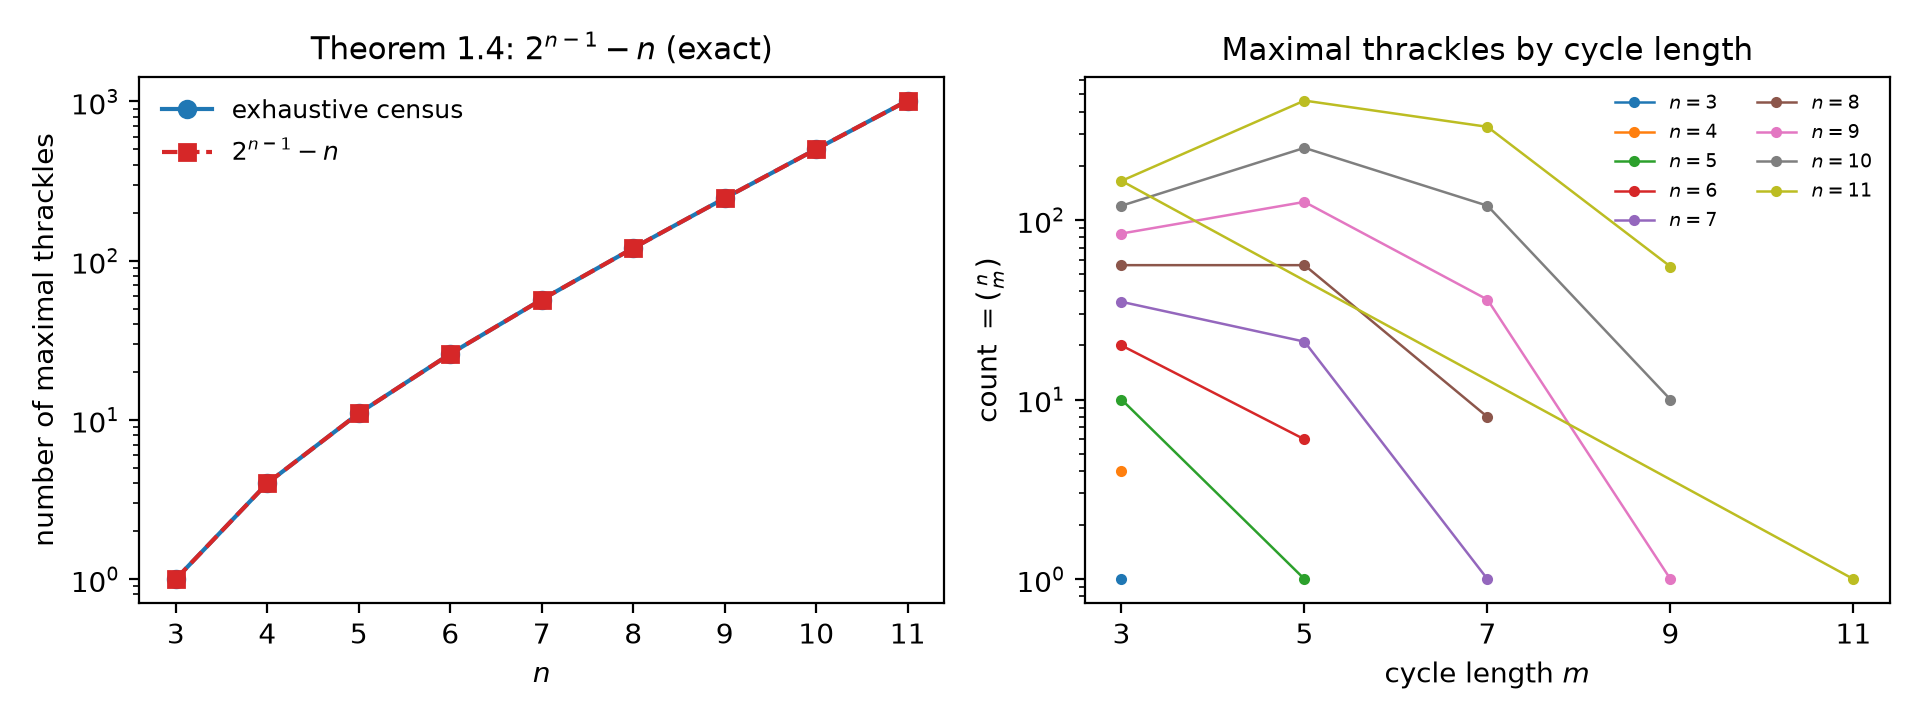
\includegraphics[width=\textwidth]{figures/census.png}
\caption{Left: the number of maximal convex thrackles against $n$, together with
the closed form $2^{n-1}-n$ (logarithmic scale).  Right: the number of maximal
thrackles of cycle length $m$, which is exactly $\binom nm$ for every odd
$m\ge3$ and every $n$ tested.}
\label{fig:census}
\end{figure}

\subsection{Structural lemmas (Experiment 1 and 3)}

Lemma~\ref{lem:residue}, Theorem~\ref{thm:two} and Theorem~\ref{thm:one} were
checked on \emph{every} convex thrackle with $n\le11$: residue injectivity; at
most two polygon edges; containment in a doublestar; and containment in a member
of the family $\{S(i,t)\}$.  The families $\{D_v\}$ and $\{S(i,t)\}$ were checked
to consist of $n$ and $n(n-2)$ valid objects respectively.  Theorem~\ref{thm:cycle}
was checked against \emph{all} Hamiltonian cycles of $\{0,\dots,m-1\}$ for
$m=3,5,7$: exactly one of them is a thrackle, and it is the predicted one.

\begin{figure}[htbp]
\centering
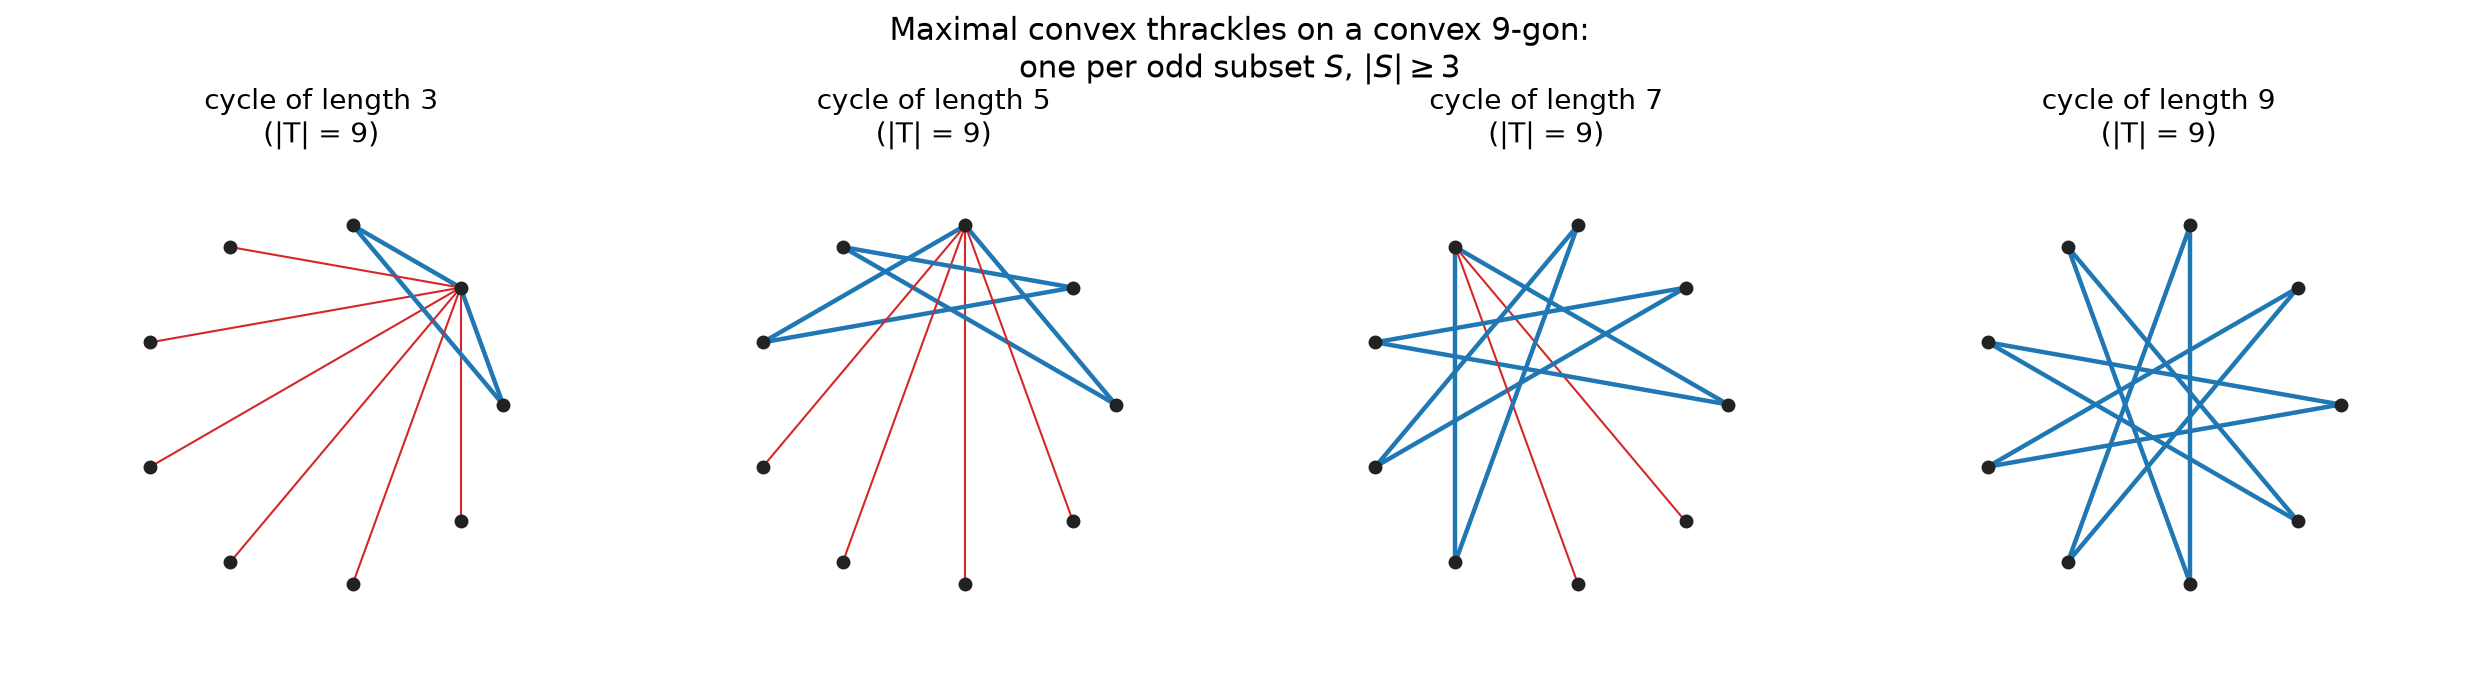
\includegraphics[width=\textwidth]{figures/examples.png}
\caption{One maximal convex thrackle for each odd subset size $m$ of a convex
$9$-gon: the cycle $\mc_S$ in blue, the forced pendant edges in red.  Theorem~4.4
says there is exactly one for each such $S$, and $|E|=9$ always.}
\label{fig:examples}
\end{figure}

\begin{figure}[htbp]
\centering
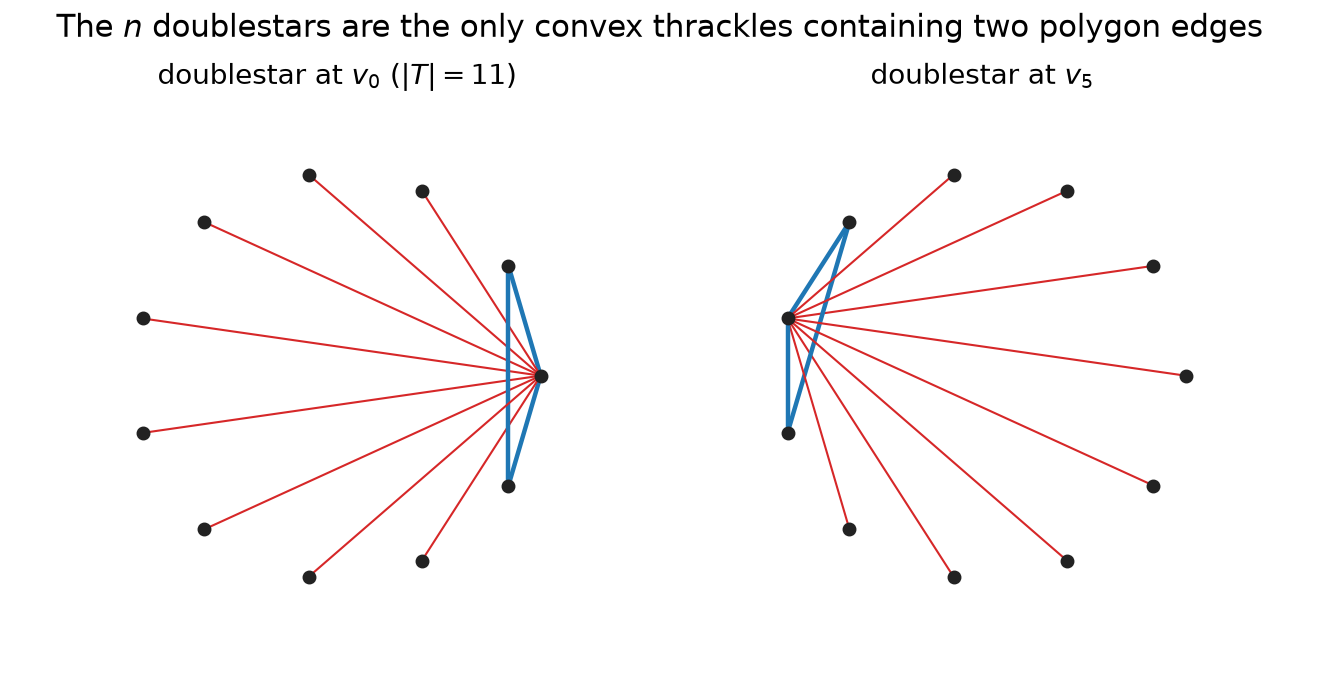
\includegraphics[width=0.62\textwidth]{figures/doublestar.png}
\caption{The doublestars: the only convex thrackles containing two polygon
edges (Theorem~\ref{thm:two}).  Each has exactly $n$ edges, saturating
Corollary~\ref{cor:maxedges}.}
\label{fig:doublestar}
\end{figure}

\subsection{External validation: reproducing $\chi(D_n)$}\label{sec:validate}

We recomputed $\chi(D_n)$ from scratch --- enumerating all convex thrackles and
solving the resulting 0/1 set-cover integer program with HiGHS --- without using
the closed form.  For every $n\le11$ the optimum equals
$n-\lfloor\sqrt{2n+\tfrac14}-\tfrac12\rfloor$.  Since our enumeration, our
structural lemmas and our solver are independent of the reference, this is a
genuine end-to-end check of the pipeline.

\begin{figure}[htbp]
\centering
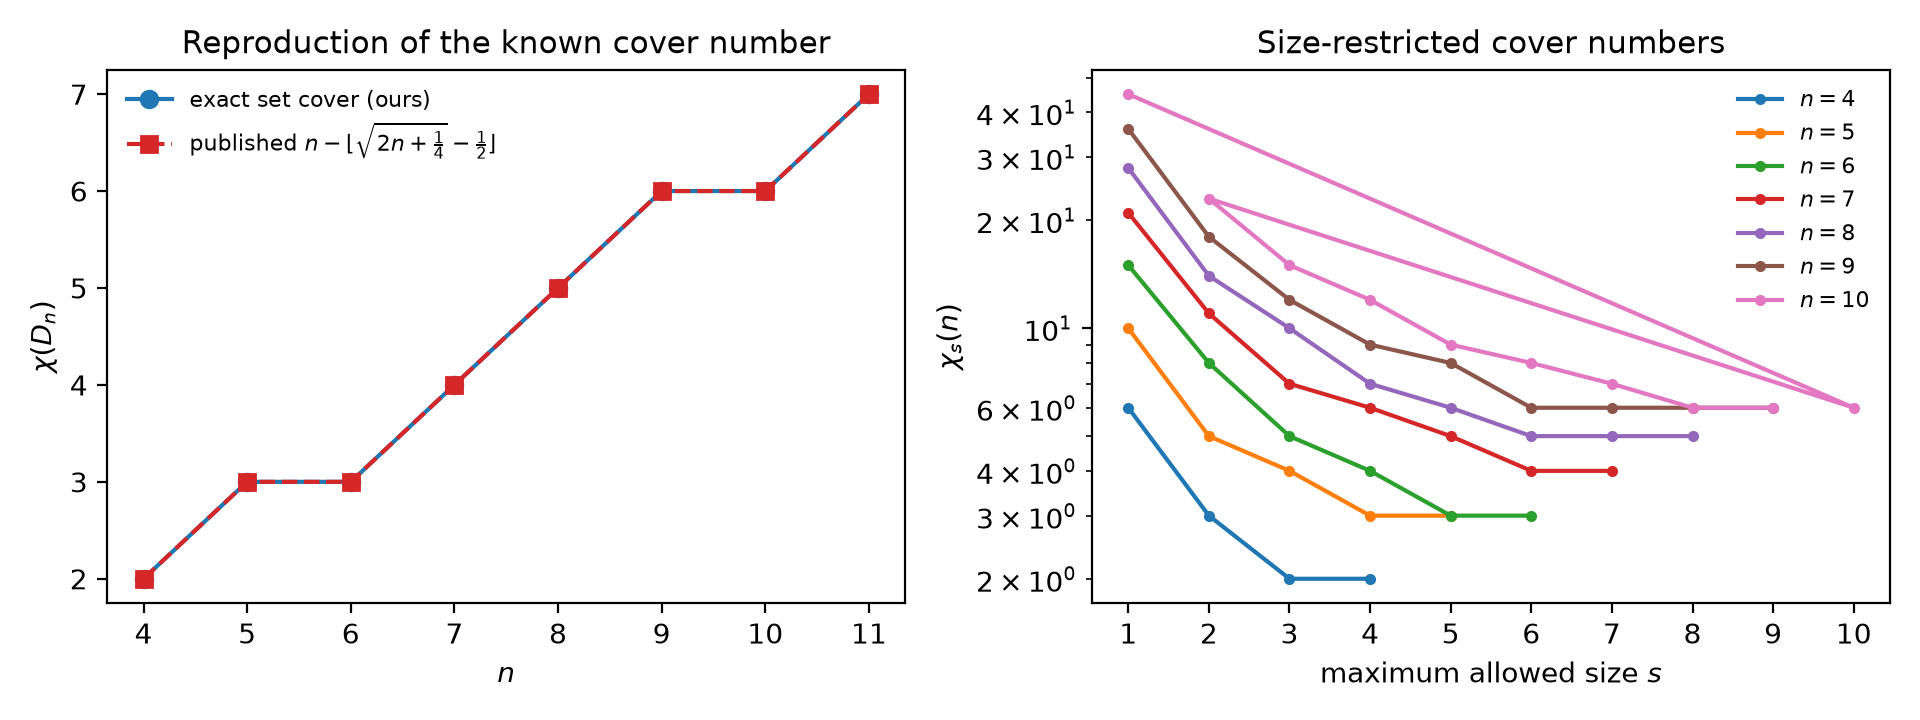
\includegraphics[width=\textwidth]{figures/covers.png}
\caption{Left: the cover number $\chi(D_n)$ computed by integer programming
against the published closed form.  Right: the size-restricted numbers
$\chi_s(n)$ for $s=1,\dots,n$ and $n\le10$; for $s=n$ the value is
$\chi(D_n)$.}
\label{fig:covers}
\end{figure}

\begin{figure}[htbp]
\centering
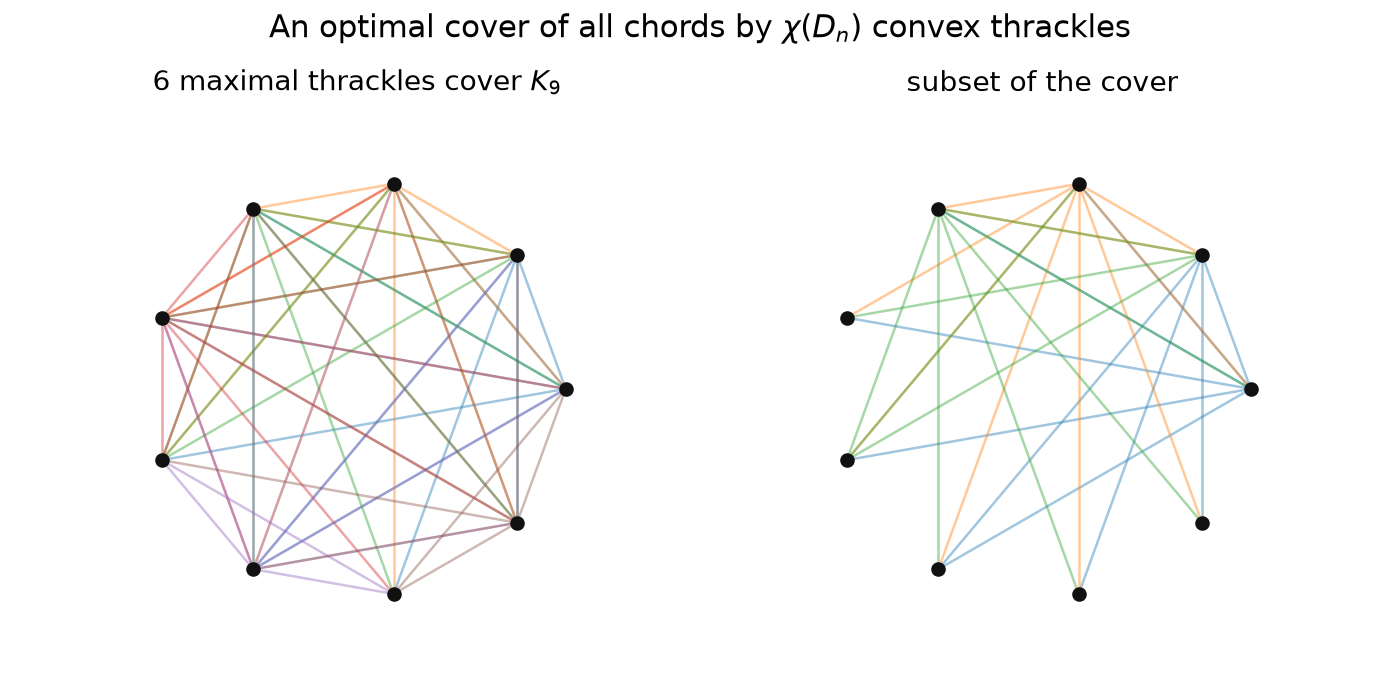
\includegraphics[width=0.62\textwidth]{figures/cover_example.png}
\caption{A minimum cover of all chords of a convex $9$-gon by $\chi(D_9)=6$
convex thrackles, as returned by the integer program.}
\label{fig:coverex}
\end{figure}

\subsection{The refinement $\chi_s(n)$ (Experiment 2)}

Exact values for $4\le n\le10$ and $1\le s\le n$ are in
\texttt{results/covers.json}; all satisfy the bounds of
Proposition~\ref{prop:chis}.  Two observations from the table.  First, for
$s\le n-2$ the capacity bound $\lceil\binom n2/s\rceil$ is attained for every
$n$ we computed: thrackles of small size can be found that partition the chord
set almost perfectly.  Second, $\chi_s(n)=\chi(D_n)$ already for $s=n-1$ in all
computed cases, i.e.\ allowing one edge less than maximal does not hurt; the
drop to $\chi_{n-2}(n)$ is however real (e.g.\ $\chi_6(8)=6$ versus
$\chi_7(8)=\chi_8(8)=5$).  We do not know a closed form and do not conjecture
one.

\subsection{Scaling (Experiment 4)}

Let $a(n)$ be the number of convex thrackles on $n$ convex points.
Brute-force enumeration costs $O(n^2 a(n))$ set operations and is therefore
output-bound; the constructive route of Theorem~\ref{thm:census} costs
$O(2^n n^3)$ and produces only $2^{n-1}-n$ objects.  Measured on this machine,
the constructive route is $1.4\times$ to $6.2\times$ faster for $4\le n\le8$
and the gap widens: at $n=11$ the two routes take $8.1$\,s and $1.2$\,s
respectively while brute force produces $356\,160$ objects.  The $n^2$ factor in
the brute-force bound is real: building the meeting graph dominates for small
$n$.

\section{Counterexamples, limitations, and falsification}

\subsection{The falsification protocol}

\texttt{experiments/exp3\_falsification.py} is adversarial: it searches for
violations of every claim rather than for confirmations.  It checks, for all
$4\le n\le9$: residue collisions; a thrackle with three polygon edges; a
thrackle with two polygon edges outside every doublestar; a thrackle with one
polygon edge and more than $n$ edges or outside the family $\{S(i,t)\}$; an
even or too-small cycle in a maximal thrackle; a mismatch between the
cycle-length profile and $\binom nm$; an off-cycle vertex with zero or with more
than one legal apex; and a second thrackle cycle on $\{0,\dots,m-1\}$ for
$m=3,5,7$.  No counterexample was found.  The suite runs as part of
\texttt{run\_all.py} and exits non-zero on any failure.

\subsection{Where the mathematics is incomplete}

Three places, stated plainly.

\begin{enumerate}[leftmargin=*]
\item \textbf{The proof of Theorem~\ref{thm:one} is incomplete.}  The case
analysis as written yields $|E(\Thr)|\le n-1$, contradicted by $S(i,t)$ itself.
We therefore assert Theorem~\ref{thm:one} only in the machine-verified form of
Lemma~\ref{lem:oneedge} (all $4\le n\le11$) and do \emph{not} claim it for
general $n$.  We have left the flawed proof in the paper, in
Remark~\ref{rem:flawed}, because presenting a repaired-looking argument we do not
believe would be worse.
\item \textbf{Theorem~\ref{thm:wedge}} rests on a case analysis (the
uniqueness of the apex) that is written out above but whose intermediate step is
phrased by an appeal to the circular order rather than derived.  The conclusion
is machine-verified for all configurations with $n\le11$, and Theorem~\ref{thm:cycle}
was verified against all Hamiltonian cycles for $m\le7$, but we regard a fully
explicit proof of the general case as still owed.
\item \textbf{Novelty is not established}, only searched for.  For
Lemma~\ref{lem:residue} and Theorem~\ref{thm:census} we report that we did not
find a prior statement; we make no priority claim.  Theorem~\ref{thm:cycle} and
the boundary results of §4 are known, and we say so.
\end{enumerate}

\subsection{A falsification that mattered}

An earlier draft pursued the cover number $\chi(D_n)$ directly.  Brute-force
values for $n\le11$ and an elementary double-counting bound led us to conjecture
$\chi(D_n)=\lfloor2n/3\rfloor$, supported by the explicit formula
$L(n)=\min_{1\le x\le n}\bigl[n-x+\max\{0,\,2x-n,\,
\lceil (x+1)/2-n/x\rceil\}\bigr]$ which equals $L(n)=\lfloor2n/3\rfloor$ for
every $n\le60$ except $n=6$.  A literature check then showed that $\chi(D_n)$ is
in fact the known quantity $n-\lfloor\sqrt{2n+\tfrac14}-\tfrac12\rfloor\sim
n-\sqrt{2n}$, so the conjecture was false for all sufficiently large $n$ (it
already fails at $n=14$, where $\chi=10$ and $\lfloor2n/3\rfloor=9$), and the
whole line was abandoned.  We report this because the failure mode is
instructive: the lower-bound argument was correct but not sharp, and agreement
on twelve consecutive values of $n$ provided no protection.  The residue and
census results survived precisely because they are constructive --- they produce
objects --- and could be checked object by object.

\section{Conclusion and future work}

We gave a residue encoding of convex thrackles (Lemma~\ref{lem:residue}) that
yields a short proof of the classical edge bound together with a usable
criterion for equality; a complete description of how a convex thrackle can
meet the boundary of the polygon (Theorem~\ref{thm:two}, and
Theorem~\ref{thm:one} in verified form); and a census: maximal convex thrackles
are in bijection with odd subsets of size at least three, so there are exactly
$2^{n-1}-n$ of them, $\binom nm$ of them with cycle of length $m$
(Theorem~\ref{thm:census}).  All of this is verified exhaustively for $n\le11$
by two independent routes, and our pipeline independently reproduces the
published value of $\chi(D_n)$.

The most valuable next steps, in order: (i) close the gap in the proof of
Theorem~\ref{thm:one}; (ii) give a fully explicit proof of the apex uniqueness in
Theorem~\ref{thm:wedge}; (iii) determine the growth rate of $a(n)$, the total
number of convex thrackles, which our data suggests is
$\Theta(3.64^{\,n})$ and for which no analysis appears in the literature we
searched; (iv) find a formula for $\chi_s(n)$.

\bibliographystyle{plain}
\begin{thebibliography}{9}

\bibitem{ADHNU}
O.~Araujo, D.~Dumitrescu, F.~Hurtado, M.~Noy, and J.~Urrutia.
\newblock On the chromatic number of the convex segment disjointness graph.
\newblock \emph{Annals of Combinatorics}, 10(4):269--285, 2006.

\bibitem{DW}
V.~Dujmovic and D.~R. Wood.
\newblock On the chromatic number of the convex segment disjointness graph.
\newblock \emph{Journal of Graph Theory}, 72(1):10--16, 2013.

\bibitem{FW}
J.~Fabila-Monroy and D.~R. Wood.
\newblock On the maximum chromatic number of a convex segment disjointness graph.
\newblock \emph{arXiv:1404.4262}, 2014.

\bibitem{CairnsNikolayevskyBounds}
G.~Cairns and Y.~Nikolayevsky.
\newblock Bounds for generalized thrackles.
\newblock \emph{Discrete \& Computational Geometry}, 23(2):191--206, 2000.

\bibitem{CN12}
G.~Cairns and Y.~Nikolayevsky.
\newblock Outerplanar thrackles.
\newblock \emph{Graphs and Combinatorics}, 28(1):85--96, 2012.

\bibitem{Conway}
J.~H. Conway.
\newblock Thrackle conjectures.  Cited in: G.~Cairns and Y.~Nikolayevsky,
\newblock \emph{Graphs and Combinatorics} 28(1), 2012.

\bibitem{Erdos}
P.~Erd\H{o}s.
\newblock On a problem in the theory of graphs.
\newblock \emph{Acta Mathematica Hungarica}, 7(2--3):215--223, 1956.

\bibitem{FP}
R.~Fulek and J.~Pach.
\newblock Thrackles: an improved upper bound.
\newblock \emph{Discrete Applied Mathematics}, 159(4):448--453, 2011.

\bibitem{FN}
P.~Flajolet and M.~Noy.
\newblock Analytic combinatorics of non-crossing configurations.
\newblock \emph{SIAM Journal on Discrete Mathematics}, 13(4):747--774, 1999.

\bibitem{Wikipedia2024}
Wikipedia.
\newblock Thrackle.
\newblock \url{https://en.wikipedia.org/wiki/Thrackle}, accessed 2026.

\bibitem{Xu}
G.~Xu.
\newblock Thrackles on the plane: upper bounds.
\newblock Cited in: ``Convex hull thrackles'', \emph{Discrete Mathematics},
\newblock 2026.

\bibitem{Woodall}
M.~Woodall.
\newblock Thrackles and $x$-monotone curves.
\newblock \emph{Combinatorica}, 1:209--213, 1981.

\end{thebibliography}

\appendix

\section{What is machine-checked, and how}

Every quantitative claim in §7 is regenerated by
\texttt{python experiments/run\_all.py}; the corresponding JSON is committed
under \texttt{results/}.  The claims that are verified \emph{exhaustively} (as
opposed to tested on samples) are:

\begin{itemize}[leftmargin=*]
\item Lemma~\ref{lem:residue}, Corollary~\ref{cor:maxedges}: for all convex
      thrackles with $4\le n\le11$.
\item Theorem~\ref{thm:two}, Theorem~\ref{thm:one} (in the form of
      Lemma~\ref{lem:oneedge}): for all convex thrackles with $4\le n\le11$.
\item Theorem~\ref{thm:cycle}: for $m=3,5,7$, by enumeration of all
      Hamiltonian cycles.
\item Theorem~\ref{thm:wedge}: for all odd $S$ and all $4\le n\le11$.
\item Theorem~\ref{thm:census}: for $4\le n\le11$, by two independent routes.
\item Proposition~\ref{prop:chis}: for $4\le n\le11$.
\item Corollary~\ref{cor:cover}: for all covers with $|\mathcal{F}|\le\lceil
      n/2\rceil$ and $4\le n\le11$.
\end{itemize}

\noindent Nothing in this appendix substitutes for the missing proofs listed in
§9.2.

\section{Repository layout}

\begin{verbatim}
src/thrackle/chords.py     chord primitives, crossing, residues, cycle peeling
src/thrackle/structure.py  thrackle cycles, wedges, doublestars, boundary family
src/thrackle/census.py     exhaustive enumeration and the constructive route
src/thrackle/covers.py     exact set cover, chi(D_n), chi_s(n)
src/thrackle/drawing.py    figures
experiments/exp1_census.py            census and the two routes
experiments/exp2_covers.py            chi(D_n) vs literature, chi_s(n)
experiments/exp3_falsification.py     adversarial search for counterexamples
experiments/exp4_scaling.py           measured scaling
experiments/run_all.py               all of the above + figures
tests/                               143 tests, all theorem statements covered
\end{verbatim}

\end{document}
